\qs{}{
    What is the average total school fees?
}

This directly adds all of the facts in the fact table since those refer to the school fees and then simply get the average of the sum.
\vspace{\baselineskip}

\sol{}
\noindent\line(1, 0){0.89\linewidth}
\begin{verbatim}
SELECT AVG(enr_tuition_fee + enr_misc_fee + enr_lab_fee + enr_ppu)
AS "Average Total School Fees" FROM enrollment;
\end{verbatim}
\noindent\line(1, 0){\linewidth}

\begin{figure}[H]
    \centering
    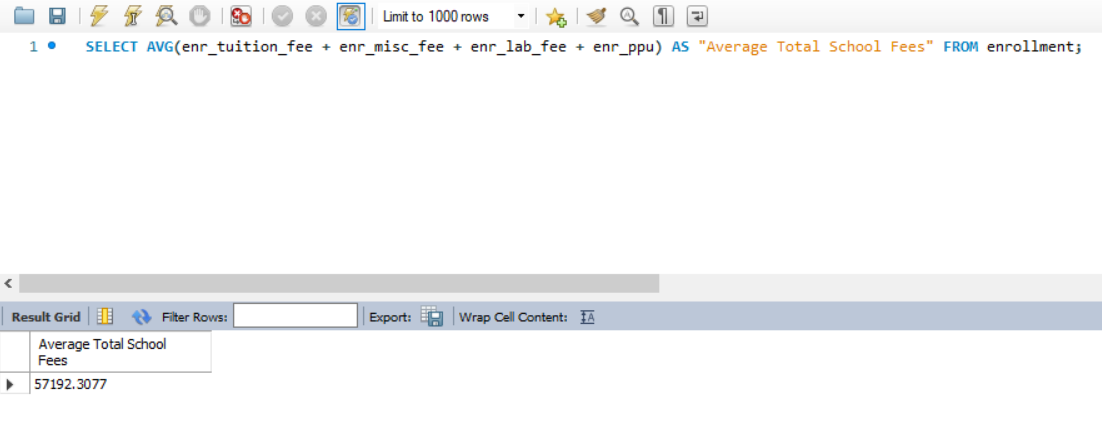
\includegraphics[width=0.7\linewidth]{images/q2.png}
    \caption{Question 2 Query and Output}
\end{figure}
